\chapter{Infraestructura y despliegue}
\label{chap:infraestructura-despliegue}

Este capítulo cubre la infraestructura cloud definida para TransitOps y el proceso de despliegue de la aplicación en AWS. Se describe la contenerización de la API con Docker, la organización modular de Terraform, la arquitectura del entorno \texttt{dev}, el flujo de despliegue paso a paso, las estrategias de rollback y restore de base de datos, la configuración DNS/HTTPS y el control de costes mediante ciclos de creación y destrucción del entorno. Los procedimientos detallados de recreación y operación se recogen en el Anexo~\ref{chap:anexo-procedimientos}.

\section{Contenerización}
\label{sec:contenerizacion}

La API se empaqueta en una imagen Docker construida a partir de su \texttt{Dockerfile}. El contenedor expone únicamente el puerto \texttt{8080}, instala las dependencias necesarias para el runtime .NET y se configura mediante variables de entorno. La imagen se utiliza tanto para despliegue cloud como para validar el comportamiento de empaquetado.

En Sprint 7 se añadió un fichero \path{.dockerignore} para reducir el contexto de construcción. Se excluyen artefactos de compilación \path{bin/} y \path{obj/}, metadatos \path{.git/}, directorios \path{.terraform/}, ficheros locales con secretos, documentación y artefactos pesados de la memoria. Esto acelera la construcción, evita transferir material innecesario al daemon Docker y reduce el riesgo de empaquetar accidentalmente información que no forma parte del runtime.

El entorno local se reproduce con Docker Compose, levantando la API y PostgreSQL. La configuración sensible se proporciona mediante un fichero \texttt{.env} no versionado. Esto permite ejecutar el sistema local sin instalar PostgreSQL de forma manual y mantiene una ruta de validación cercana al despliegue real.

\section{Infraestructura como código}
\label{sec:infraestructura-codigo}

Terraform se organiza bajo \path{infra/terraform}. La estructura separa un bootstrap de estado remoto, módulos reutilizables y raíces de entorno:

\begin{itemize}
  \item \path{bootstrap/remote_state}: crea el bucket S3 de estado y la tabla DynamoDB de bloqueo.
  \item \path{modules/platform_foundation}: VPC, subredes, rutas, NAT y grupos de seguridad.
  \item \path{modules/container_registry}: repositorio ECR.
  \item \path{modules/database}: RDS PostgreSQL.
  \item \path{modules/runtime_config}: Secrets Manager y SSM.
  \item \path{modules/container_runtime}: ECS, task definition, ALB, listeners, Route 53 y ACM.
  \item \path{modules/observability}: grupo de logs, dashboard CloudWatch, alarmas y notificación SNS opcional.
  \item \path{modules/github_oidc}: rol de despliegue para GitHub Actions.
  \item \path{environments/dev}: composición real del entorno de desarrollo.
\end{itemize}

El estado remoto se almacena en S3 y se bloquea con DynamoDB. Esto evita estados locales divergentes y reduce el riesgo de cambios concurrentes.

\section{Entorno AWS}
\label{sec:entorno-aws}

El entorno desplegado utiliza:

\begin{itemize}
  \item Cuenta AWS: \texttt{661000947340}.
  \item Región: \texttt{eu-west-1}.
  \item Entorno: \texttt{dev}.
  \item Dominio objetivo validado: \endpoint{api.dev.transitops.net}.
  \item Hosted zone: \path{transitops.net} en Route 53.
  \item Identificador de hosted zone: \path{Z0844787W37HXN9FIJR}.
  \item Fallback operativo: DNS público del ALB cuando el entorno se recrea antes de completar DNS/ACM.
\end{itemize}

Los recursos siguen la convención \path{transitops-dev-<componente>} y se etiquetan con proyecto, entorno, propietario, repositorio, servicio, origen Terraform y las etiquetas \texttt{TerraformStack} y \texttt{ResourceGroup}. Esta nomenclatura permite identificar recursos y costes, y comprobar tras un \texttt{terraform destroy} que no quedan recursos del entorno \texttt{dev}.

Como el entorno \texttt{dev} es educativo y desechable, la configuración actual desactiva la retención automática de backups de RDS y omite snapshots finales. Esta decisión reduce costes residuales en ciclos frecuentes de creación y destrucción, sin impedir que un entorno futuro de producción defina una política de backup más conservadora.

\section{Despliegue de la aplicación}
\label{sec:despliegue-aplicacion}

El flujo de despliegue aplicado en \texttt{dev} durante la primera validación cloud fue:

\begin{enumerate}
  \item Crear la infraestructura base con ECS en \texttt{desired\_count} = \texttt{0}, evitando arrancar tareas antes de tener imagen en ECR.
  \item Construir la imagen Docker de la API.
  \item Publicar la imagen en ECR con el tag \path{sprint4-local-d00aa6b}.
  \item Actualizar la task definition para usar la imagen publicada.
  \item Cargar los secretos de runtime en Secrets Manager.
  \item Ejecutar migraciones con una tarea ECS puntual usando \path{--migrate-only}.
  \item Escalar el servicio ECS a \texttt{desired\_count} = \texttt{1}.
  \item Activar Route 53, ACM, HTTPS y redirección HTTP a HTTPS.
  \item Validar el endpoint público de readiness sobre HTTPS.
\end{enumerate}

En Sprint 6 se repitió la recreación del entorno en la cuenta AWS actual \texttt{661000947340}. La imagen validada fue \path{sprint6-local-6bb910c}; se restauraron e importaron secretos que habían quedado programados para eliminación tras un ciclo anterior, se ejecutó una tarea ECS de migración con código de salida \texttt{0}, se escaló el servicio a \texttt{desired = 1} y se validaron readiness, bootstrap de administrador y login. La validación funcional principal de Sprint 6 se hizo mediante el DNS HTTP del ALB, y posteriormente se corrigió la delegación DNS de \path{transitops.net} en la misma cuenta para que el siguiente \texttt{terraform apply} pueda converger directamente con \texttt{enable\_https = true}.

El módulo de runtime incluye además el deployment circuit breaker de ECS con rollback, periodo de gracia para health checks y parámetros explícitos para la comprobación del target group: ruta \path{/api/v1/health/ready}, intervalo, timeout y umbrales de healthy/unhealthy. Esto reduce el riesgo de dejar una versión fallida recibiendo tráfico.

Sprint 7 completó este hardening con un \texttt{stopTimeout} explícito de \texttt{30} segundos en la task definition, un \texttt{deregistration\_delay} corto en \texttt{dev}, y cadenas de conexión cloud con timeouts y pooling configurados de forma explícita. El objetivo no es optimizar rendimiento en abstracto, sino hacer más predecible el arranque, la parada y la ejecución puntual de migraciones en ECS. La validación real usó la imagen \tech{sprint7-good-3dca035}, ejecutó migraciones con exit code \texttt{0} y dejó temporalmente el servicio en \texttt{desired = 1} y \texttt{running = 1} antes del cierre de coste.

\section{Rollback y restore}
\label{sec:rollback-restore}

La recuperación ante despliegues fallidos se resolvió de forma coherente con el resto del proyecto: Terraform sigue siendo la fuente de verdad. El rollback manual se ejecuta reaplicando el entorno con un tag de imagen conocido, por ejemplo \tech{sprint7-good-3dca035}, y manteniendo \texttt{ecs\_desired\_count = 1}. El workflow \path{rollback-dev.yml} automatiza esta operación y comprueba después que ECS queda estable y que el health check responde correctamente.

También se ejecutó una prueba controlada de fallo usando el tag inexistente \tech{sprint7-missing-3dca035}. Este escenario forzó un error de despliegue por imagen no disponible, permitió observar los eventos de ECS y demostró el comportamiento del deployment circuit breaker. La tarea falló con \texttt{CannotPullContainerError}. Tras la prueba se reaplicó el tag bueno \tech{sprint7-good-3dca035} para que el estado de Terraform y la task definition volvieran a quedar alineados, y el readiness respondió de nuevo \texttt{200}.

Para la base de datos, \texttt{dev} mantiene \texttt{database\_backup\_retention\_days = 0} y no genera snapshots finales al destruirse. La fiabilidad se valida mediante snapshot manual: el script \path{scripts/cloud/aws/Invoke-RdsRestoreTest.ps1} crea un snapshot de la base principal, restaura una instancia temporal, crea un secreto temporal con la cadena de conexión restaurada, registra una task definition temporal y ejecuta \path{--migrate-only} contra esa base. El criterio de éxito es código de salida \texttt{0}. Salvo que se active una opción para conservar evidencia, el propio script elimina la base restaurada, el secreto, la task definition temporal, la política IAM temporal y el snapshot manual. La Figura~\ref{fig:rollback-restore} recoge la evidencia de ambas pruebas: el rollback automático con recuperación al tag correcto y la tarea de migración finalizada correctamente contra la base restaurada.

\begin{figure}[htbp]
\centering
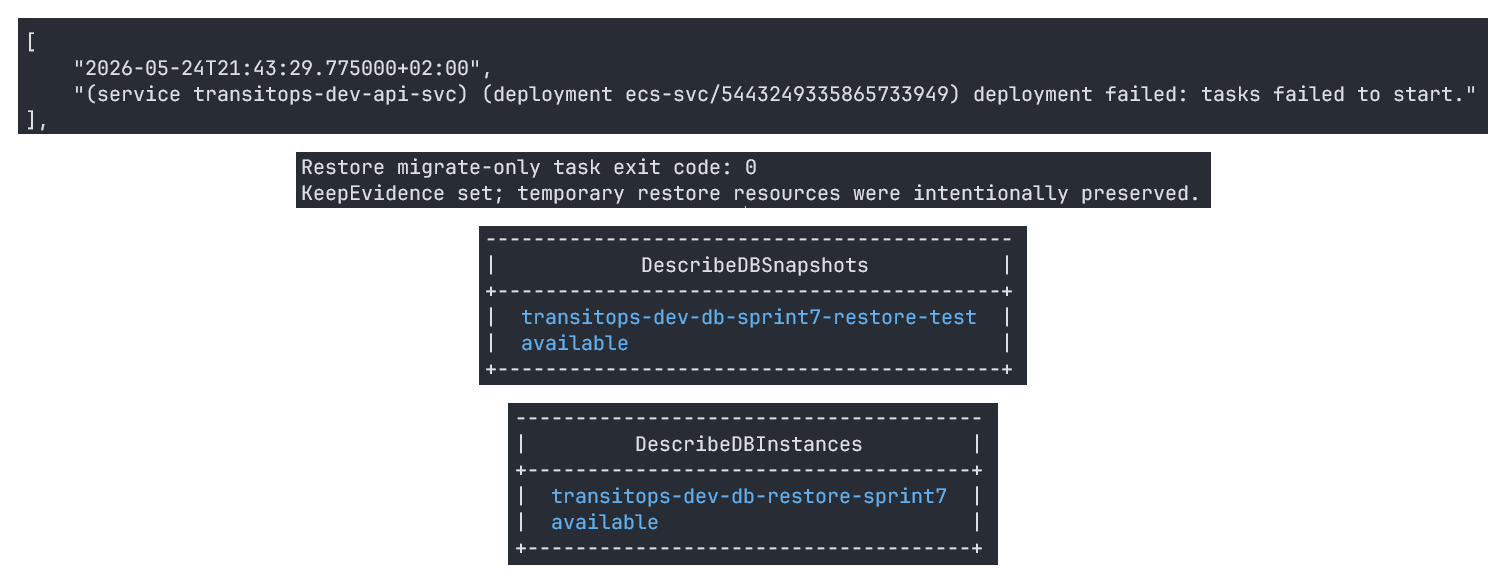
\includegraphics[width=0.92\textwidth]{imaxes/rollback-restore-evidence}
\caption{Evidencia de rollback automático y restore real de RDS.}
\label{fig:rollback-restore}
\end{figure}

\section{DNS, certificados y HTTPS}
\label{sec:dns-certificados-https}

El endpoint objetivo es \endpoint{https://api.dev.transitops.net}. Para lograrlo, Terraform solicita un certificado público en ACM para \endpoint{api.dev.transitops.net}, crea el CNAME de validación en Route 53, espera a que el certificado pase a estado \texttt{ISSUED}, crea el listener HTTPS \texttt{443} en el ALB y convierte el listener HTTP \texttt{80} en una redirección permanente hacia HTTPS.

Durante la activación en la cuenta \texttt{661000947340} apareció una incidencia real de DNS: el dominio registrado \path{transitops.net} apuntaba a nameservers distintos de los de la hosted zone usada por Terraform. ACM permanecía en \texttt{PENDING\_VALIDATION} aunque el CNAME existía en Route 53, porque el DNS público no consultaba esa zona. La corrección consistió en actualizar los nameservers del dominio registrado para que coincidieran con la hosted zone \path{Z0844787W37HXN9FIJR}. Tras la propagación, el CNAME de validación fue visible desde DNS público y el certificado pasó a \texttt{ISSUED}, como se muestra en la Figura~\ref{fig:acm-issued}.

\begin{figure}[htbp]
\centering
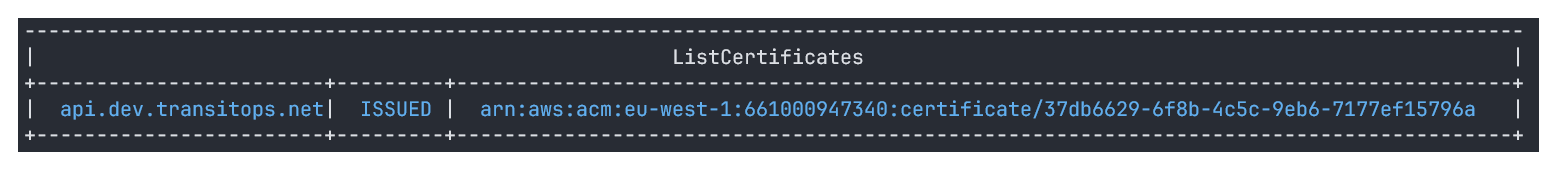
\includegraphics[width=0.92\textwidth]{imaxes/acm-issued}
\caption{Evidencia del certificado ACM emitido para el endpoint de desarrollo.}
\label{fig:acm-issued}
\end{figure}

\section{Cierre del entorno y control de costes}
\label{sec:cierre-costes}

Después de capturar la evidencia de Sprint 6, el entorno \texttt{dev} se destruyó con \texttt{terraform destroy} para evitar gasto evitable. La destrucción eliminó ALB, listeners, certificado ACM, registros DNS de \endpoint{api.dev.transitops.net}, ECS, ECR, RDS, NAT Gateway, VPC, subredes, grupos de seguridad, CloudWatch logs, dashboard, alarmas y secretos del entorno. El repositorio ECR necesitó una limpieza previa de imágenes, ya que AWS no permite eliminar un repositorio no vacío.

En Sprint 7 se ajustó el módulo de ECR para permitir \texttt{force\_delete} en \texttt{dev}. Esta decisión evita que una imagen publicada para validar rollback bloquee el destroy final. El ajuste es deliberadamente parametrizable para que un entorno productivo pueda conservar una política más restrictiva.

Tras el destroy de Sprint 7, Terraform informó \texttt{72 destroyed}. Se verificó que el state quedaba vacío y que no existían recursos costosos asociados al stack \path{transitops-dev}: ALB, RDS, ECS, ECR, certificado ACM, registros DNS del subdominio, log groups, dashboards, alarmas, snapshots temporales ni secretos. El NAT Gateway quedó en estado \texttt{deleted}. Permanecen fuera del destroy el dominio registrado \path{transitops.net}, la hosted zone pública y los recursos de backend remoto de Terraform, que son recursos base de bajo coste y necesarios para recrear el entorno.

\section{Gestión de configuración y secretos}
\label{sec:configuracion-secretos}

La configuración sensible se externaliza. La cadena de conexión a PostgreSQL, la clave de firma JWT y el token de bootstrap se almacenan en Secrets Manager. Otros parámetros, como emisor, audiencia y expiración del JWT, se almacenan en SSM Parameter Store o se proporcionan como variables no secretas.

En el repositorio solo se incluyen ejemplos y nombres de variables. Los ficheros locales que pueden contener secretos, como \texttt{terraform.tfvars}, \texttt{backend.hcl} o \texttt{.env}, están excluidos del control de versiones.
